\chapter{Functional Objectives and Existing Solutions}

\section{Usage Scenarios}
\subsection{Asking for Help}
Having the possibility to ask for help is a vital part of the working culture in many knowledge driven
businesses, so collaboration and the sharing of ideas are a major factor in the company guidelines
of SinnerSchrader. The application is supposed to act as a central repository for knowledge and contacts,
enabling employees to find someone who can help in order to answer questions and find solutions to domain-specific problems.

\subsection{Finding Potential Team Members}
Team managers constantly face the problem of reassembling parts of their teams, forming new teams for new projects, and
disbanding teams whose projects have ended. As there is no unified source of information about all employees at SinnerSchrader, managers often
do not find the best suitable team member to fill an open position because they simply do not know each other yet.
The tool will give managers the opportunity to search the entirety of employees at SinnerSchrader and find one
meeting all requirements of the open position, thus making collocating teams easier and more efficient.

\subsection{Collecting Information}
The application will give employees the possibility to provide information about their personal knowledge regarding their skills.
Furthermore, they can assign a will value for every skill that describes if they prefer
doing the implicitly linked activity or working with the tool described by said skill. That is, people can define what they want to do and what tasks they would like to refuse.\\
As employees continually enlarge their knowledge while their fields of interest shift towards new technologies, tools or even
functional divisions, providing data about their skills and preference once will lead to the system being filled with obsolete
information. The quality of the search results and suggestions heavily relies on the fidelity and volume of the underlying data about the employees, hence keeping said information up to date is crucial to the performance of the application.

\subsubsection{Biannual Feedback Meetings}
Every employee has biannual meetings with their respective supervisor to interchange
bidirectional feedback, define personal goals, and negotiate possible changes of salary.
Part of the feedback given by the employee are subjects they learned or enhanced their knowledge about, and newly developed interests. These insights are documented and registered in the employee's personnel file.
This meeting will be the regular occasion for supervisors and employees to refine the data saved in the application and to add
newly gained skills to it. The supervisor is advised to address discrepancies between the employee's and their own estimations of skills to accommodate the human factors of self-perception. A case study performed by Beck indicates that this approach to
collect information about the employees' skills generates a sufficient amount of data to run such a system \cite{beck}.

\subsection{Notifications by Supervisors}
Employees and supervisors are encouraged to be in rich contact with each other in order to deliver continuous feedback
about the individual person's needs, impediments, and the status of their current projects.
As a result, supervisors can identify appropriate moments for reevaluating the skills and preferences saved in the application and notify the employee.\\
For example, according to Tuckman's team development model, the so called \textit{adjourning} phase of a project is an occasion for ``recognition of individual achievements and reflection on how far the team has come'' \cite[P. 3]{Wilson} and thus is a convenient chance to add new skills acquired during the project and to refine the existing data.

\subsubsection{Automatic Notifications}
In contrast to the supervisor, the application cannot be able to find the best situations to notify employees to maintain their skill profile, so sending automatic notifications will not be nearly as effective as being reminded by the supervisor. Furthermore, according to the \textit{Direct Marketing Association (UK)}\footnote{https://dma.org.uk/}, only
about one in five automatically generated e-mails will be opened \cite{mailrep}, which reflects SinnerSchraders
experiences with email reminders. Those facts justify the decision, that the system will not send any notification to its users.

\newpage
\subsubsection{Intrinsic Motivations}
In addition to the mentioned reasons for employees to provide data about their skills which are all extrinsic motivations,
there also exist intrinsic motivations to do so. Being motivated intrinsically is defined as ``doing something because it is inherently interesting or enjoyable'' \cite{RYAN200054}. As people are motivated to focus on tasks they fancy, they are also motivated to voluntarily keep an eye on the quality of the data that is used to determine the tasks they will have to perform.


\section{Requirements}
\label{requirements}
\subsection{Functional Requirements}
\begin{itemize}
 	\item Accessible to all Employees\\
	Every employee must be able to use the application regardless of their equipment or preferred operating system.
	\item User Profiles \\
	Anyone can see another user’s profile consisting of basic information about the user such as name, location, e-mail and personal skills. Personal skills are composed of a name, a skill level and a will level, both on a scale from one (worst) to four (best).
	\item Provide/Edit skills\\
	Users can add new skills from a pool of known skills to their own profile. Already added skills can be edited and removed from the profile.
	\item Search\\
	A search function can be used to find people who have added one or more specific skills to their profile. When searching for multiple skills, only persons matching all of them will be displayed.
	\begin{itemize}
		\item Ranking\\
			By default, the search results' order should be defined by a score aggregating the individual employee's skill level, will level and grade of specialization in the searched skills.
		\item Sorting\\
			The user should be able to sort the search results not only by said score
			but also by knowledge and will level.
	\end{itemize}
	\item Management of Known Skills\\
	New skills can be added to the set of known skills in the application. Existing skills can be edited and removed. Users' personal skills are automatically updated when a skill has been edited, so that the integrity of the users' profiles is maintained at all times.
\end{itemize}

\subsection{Non-Functional Requirements}
\begin{itemize}
	\item Device Types\\
		Even tough smartphones are gaining more and more share in terms of total internet traffic \cite{allthemobile},
		the application will be optimized for desktop use. Every employee has permanent access to their computer and uses it
		for their work, so it is assumed, that the very same machines will be used to access the skill management application.
	\item Browsers\\
		Every employee is allowed and encouraged to install their favorite software on their personal computer, so nearly every web browser can be found.
		The application should run on \textit{Google Chrome}\footnote{https://www.google.com/chrome/browser/desktop/index.html}, \textit{Mozilla Firefox}\footnote{https://www.mozilla.org/en-US/firefox/products/} and \textit{Safari}\footnote{http://www.apple.com/lae/safari/} in their latest versions. \textit{Internet Explorer}\footnote{https://www.microsoft.com/en-us/download/internet-explorer.aspx} and \textit{Edge}\footnote{https://www.microsoft.com/en-us/windows/microsoft-edge} will not be supported.
	\item Scalability\\
		SinnerSchrader has 459 full-time employees \cite{quartalsbericht}, so the application will be designed for approximately 500 users. In the event of a rapid growth in the userbase, e.g. due to the opening of another office, the system will have to scale up to handle the larger number of users.
	\item Load/Response Times\\
	\label{require_times}
		According to \textit{Google's} RAIL model, a website needs to respond to the user's input within 100ms to offer a fluent user experience; the triggered action should be finished within one second after the user's interaction \cite{RAIL}. In the context of the application's search function, this means that the system will show the user that their input has been acknowledged within 100ms. Within one second after the submission of the search request, the result list will be rendered completely.
\end{itemize}



\section{Commercial Solutions}
\label{commercial}
Three commercial skills management applications have been picked randomly for further examination: \textit{Skills Base}, \textit{engage! Talent Management} and \textit{SkillsDB Pro}.
A more detailed analysis by Lehner shows that most tools provide a spectrum of features and limitations very similar to the examined solutions \cite{Marktanalyse}, so that the selection is assumed to be representative of the market.

\subsection{Skills Base}
Skills Base\footnote{http://http://www.skills-base.com/} offers the required features, but also includes a large number of functionality SinnerSchrader does not need and is not willing to use. This includes assessments, the categorization of skills, and a role model for advanced access rights configuration.
The search function does not provide searching for multiple skills. Furthermore, the sorting of results found cannot be customized. A central point of the application are dashboards displaying information about the most popular skills in the organization and long term statistics.
\begin{figure}[!htp]
    \centering
    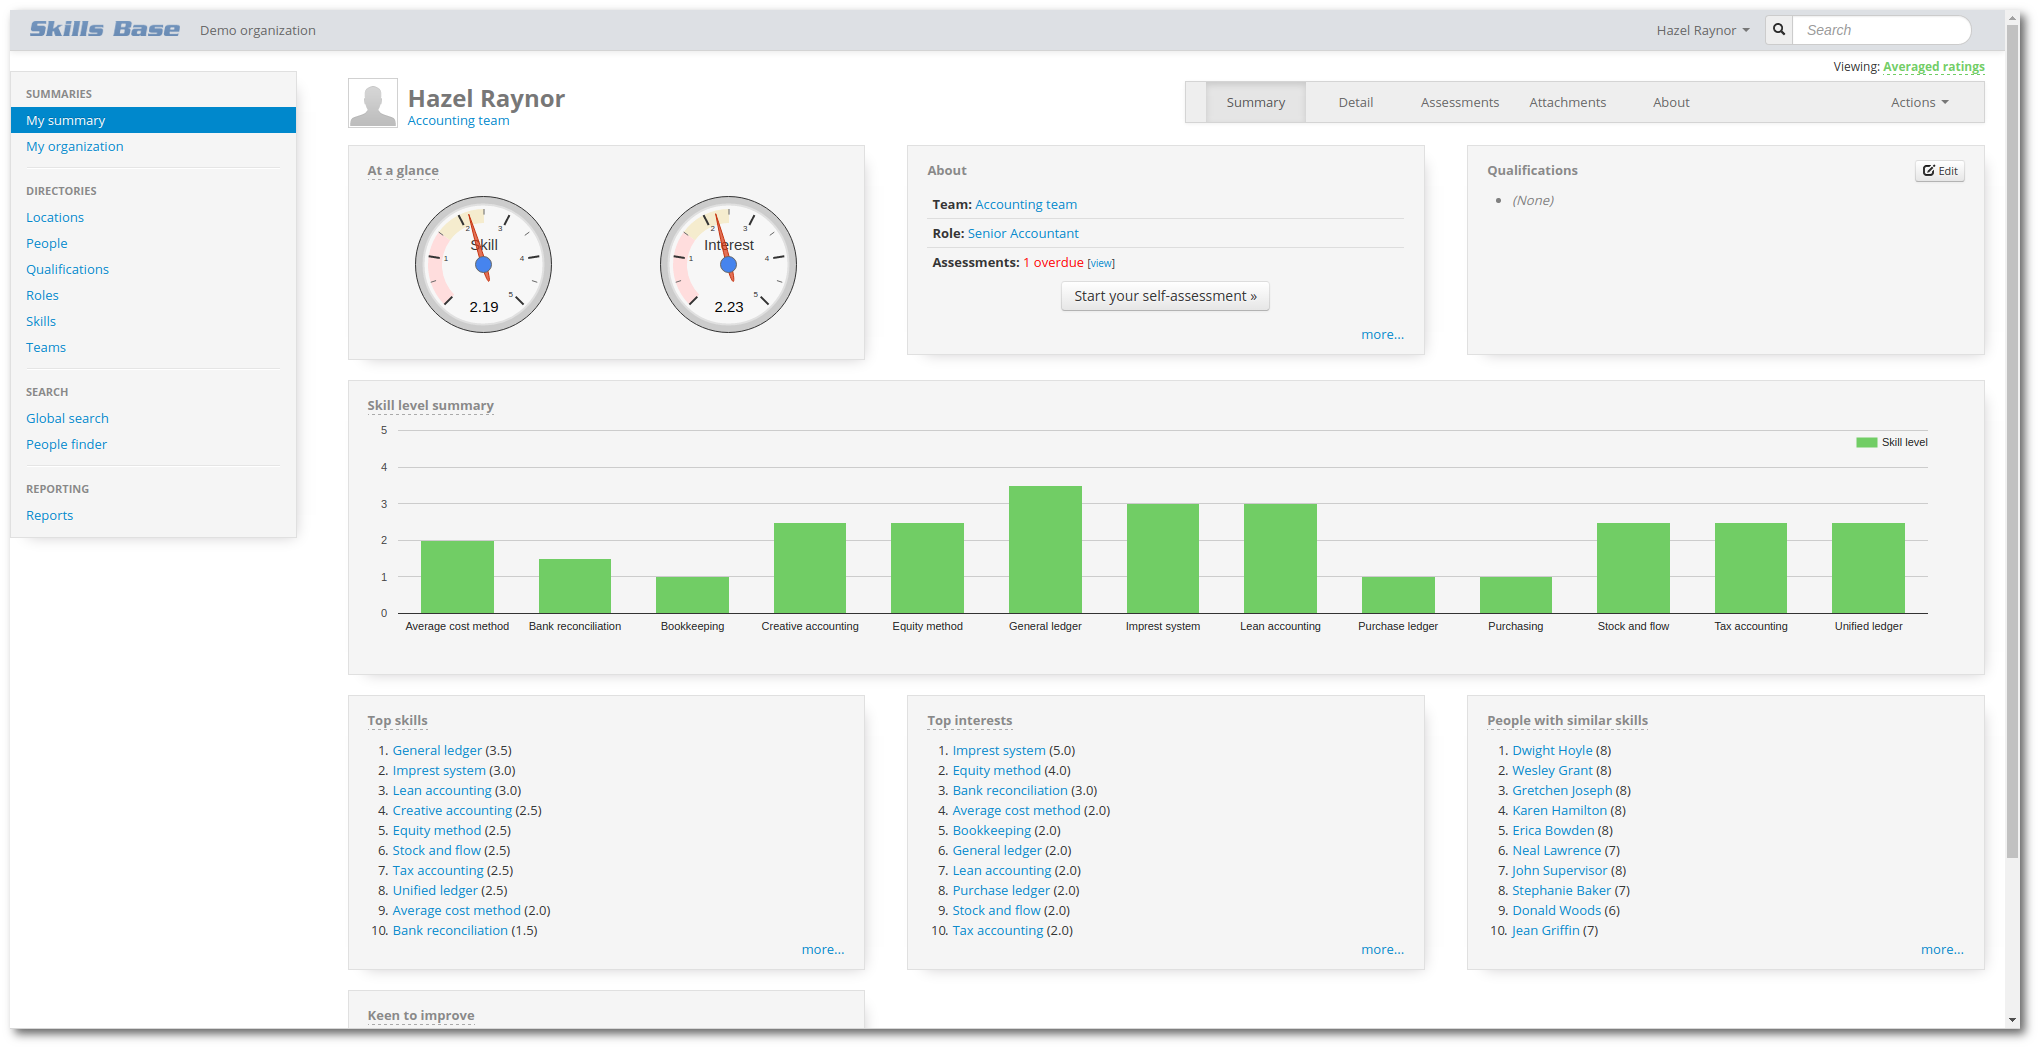
\includegraphics[width=\textwidth]{images/skillsbase-dashboard.png}
    \caption{SkillsBase Dashboard}
    \label{fig:skillsbase_dashboard}
\end{figure}

\subsection{Talent Management (engage!)}
Talent Management\footnote{http://www.infoniqa.com/hr-software/skill-management} is a module for Infoniqa’s management software engage!\footnote{http://www.infoniqa.com/hr-software/personalmanagement}. It offers advanced features for managers such as a powerful search function controlled via a special query language. It also includes data about the employees’ salaries, feedback protocols, and certificates. It can only be used in combination with engage!, a complete human resources management solution including features like time tracking, e-learning, applicant management and payroll accounting.

\begin{figure}[!htp]
    \centering
    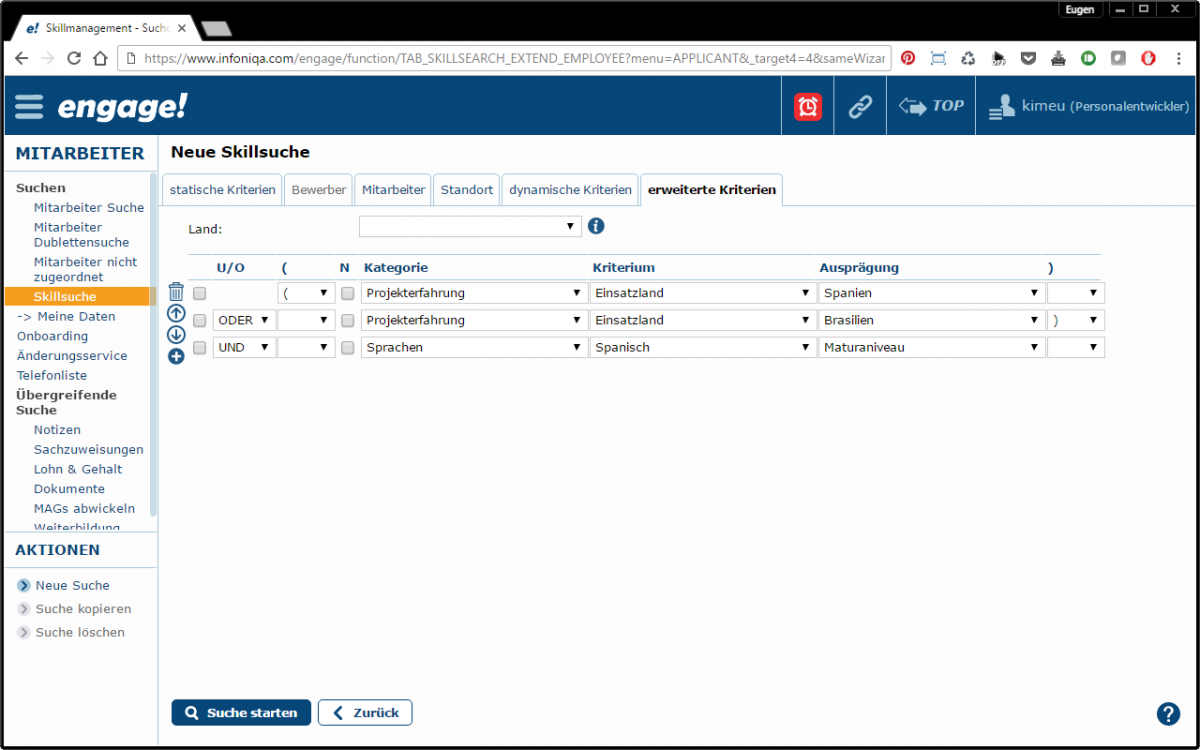
\includegraphics[width=\textwidth]{images/talent_management_-_skillmanagement_-_skillsuche.png}
    \caption{Talent Management Search}
    \label{fig:talent_management}
\end{figure}

\subsection{SkillsDB Pro}
SkillsDB Pro\footnote{http://www.skillsdbpro.com} is an application designed to serve as a database in an organization providing an overview of every person’s own skills and training only to themselves and their manager. The search function is capable of searching for multiple skills combined with different logical operators which enables users to enter very sophisticated queries.
Not only can users provide information about their skills, but managers can also do this with the limitation that no employee can see their manager’s rating about themselves.
Furthermore, only managers can search for persons. Taking into consideration that SinnerSchrader needs a tool to enable everyone to find someone with a specific skillset, this is a serious disadvantage.
SkillsDB also offers features SinnerSchrader does not intend to use including the automatic generation of project reports based on plan succession and demands for assessments.

\subsection{Conclusion}
None of the analyzed applications offers all features required, but all of them include various functions SinnerSchrader does not intend to use, which brings undesired complexity into the applications.
One of the most critical features, sorting the search results by both knowledge and motivation is not offered by any of the commercial solutions.
Furthermore, all those systems differentiate between employees and their supervisors and thus restrain transparency. The application is not supposed to be used for monitoring and rating employees, but should give employees the possibility to find each other; categorizing them would clearly defeat this purpose.

\subsubsection{Pain Point Fitness Scoring}
As shown by Canós‐Darós, motivation is a vital factor regarding any employee's performance and quality of work \cite{CanosDaros2013}.
Although motivation is a complex construct of many highly diverse dimensions, the overlap of a person's interests and their duties is a key aspect to it.
Assuming that every member of the company has some skills they prefer to employ over others, matching people to tasks that require the exact same abilities they are interested in employing will lead to more motivated employees and thus have a positive impact on the overall productivity.
Consequently, when searching for persons having specific skills, the application should not only take into account the employees' skills but also their preferences in order not to find the most skilled, but the best fitting one. Unfortunately, none of the examined applications does provide a way to aggregate both skills and preferences into a single score indicating the overall grade suitability of a person relative to the searched skills.
